\documentclass{ximera}

%% Where to find images
\graphicspath{  %% When looking for images,
{./}            %% look first at your level,
{./basics/}     %% then in this folder,
}    

\title{Common use cases}
\author{Bart Snapp}

\begin{document}
\begin{abstract}
  We'll discuss common ways people use Ximera.
\end{abstract}
\maketitle

There are many ways our friends use Ximera. Some make worksheets, some make
exercise banks, and some make full textbooks. Common to all of these are the
use of interactive elements that students submit answers to. We'll call
anything a student can \textit{answer} an \textbf{answerable}.

\begin{warning}
  All answerables must be \textbf{inside of a theorem-like environment}.
\end{warning}

With that said, we'll discuss the basic answerables below, and then described
how they might be used in use cases of: worksheets, exercise banks, and
textbooks.

\section{The \texttt{\textbackslash answer} command}

The basic way of including a answerable item in Ximera is to use the
\verb|\answer| command.

\begin{warning}
  The \verb|\answer| command must be in \textbf{math-mode} (display or inline)
  and also be \textbf{inside of a
    theorem-like environment}.
\end{warning}
Here are some examples of how to use \verb!\answer!. We can validate a single
number:
\begin{verbatim}
\begin{problem}
State the answer to life, the universe, and everything.
\[
\answer{42}
\]
\end{problem}
\end{verbatim}
We can validate an expression of variables:
\begin{verbatim}
\begin{exercise}
Compute:
\[
\frac{\partial}{\partial x} \sin(3xyx) 
= \answer{3yz\cos(3xyz)}
\]
\end{exercise}
\end{verbatim}
We can validate with several answerables in an environment:
\begin{verbatim}
\begin{question}
For each of the following functions, find $x$ such that it is a
critical point, or write ``NA'' if none exists.
\begin{enumerate}
  \item For $f(x) = |x-4|$, $x$ is a critical point when 
  $x=\answer{4}$.
  \item For $g(x) = x^2-4x+1$, $x$ is a critical point when 
  $x=\answer{2}$.
  \item For $h(x) = 3x-2$, $x$ is a critical point when 
  $x=\answer[format=string]{NA}$.
\end{enumerate}
\end{question}
\end{verbatim}

There are also a number of optional arguments that can be passed
to the \verb|\answer| command.
\begin{description}
  \item[\tt\bfseries tolerance] sets a $\pm$ value on the
    author's (numeric) answer that will be accepted from a student. For
    example,
    the answer box \verb|\answer[tolerance=5]{100}| will accept anything in
    the range of $[95,105]$ as correct.
  \item[\tt\bfseries format=string] validates \textit{words} typed into an
    answer box. Here \verb|$\answer[format=string]{Cat}$| will validate
    \verb!Cat!,
    \verb!cAt!,\verb!caT!, \verb!cat! all as
    correct. However, if spaces are inserted before, between, or after, it will
    be marked as incorrect.
  \item[\tt\bfseries given] will show an answer in the PDF. Sometimes it is
    necessary to
    show such content to ensure
    understandable in a PDF setting. Here \textit{given} means
    that the answer is \textit{given} to the student in the PDF.
\end{description}
There are two other optional arguments \verb!validator! and \verb!id!, but they
are for building custom validators and are beyond the scope of this document.

\begin{warning}
  You separate options in \verb!\answer! using commas and there can be no
  spaces, like this:
  \begin{verbatim}
\[
\answer[given,tolerance=5]{100}
\]
\end{verbatim}
\end{warning}

\paragraph{Validating an answer} is achieved by client-side JavaScript. Around
one dozen algorithms to check if the student's provided
answer is mathematically equivalent to the content author's provided answer. If
any report the answer as being correct, then it is marked as correct.

\begin{warning}
  There are confounds for validating answers online:
  \begin{description}
    \item[Student input] for answers a nontrivial task. Students need to be
      able
      to easily type in their answers.
    \item[Checking for equality] will not reveal the form of the answer. This
      means that sometimes the \textit{answer} to the question can be the
      question
      itself. For example  \verb!1+2 = \answer{3}! can be answered with `$1+2$'
      because
      that \textit{equals} $3$.
    \item[Right-click reveals the answer] to the students. Moreover, the source
      is open to the students. Ximera is not designed for high-stakes
      assessment.
      \item[Richardson's theorem ]\link[states it is not
        possible]{https://en.wikipedia.org/wiki/Richardson\%27s\_theorem}
      to decide equality between the expressions of involving integers, $\pi$,
      logarithms and exponential and sine functions.
    \item[Floating-point numbers] can lead to erroneous computations, leading
      to
      identifying nonequal expressions as equal.
  \end{description}
\end{warning}
In abstract, each of these confounds are quite daunting. However, in practice,
they can be mitigated via Ximera's design along with thought on the author's
side when constructing problems.

\paragraph{Student input} is reflected back to the student, in the sense that
Ximera tells the users what it thinks they are typing.
In addition, we provide a math
pallet. Authors can assist students with input by ensuring that the required
answer is not too difficult to type in.

\paragraph{Ximera checks for equality} and is comprehensive in
practice, but that can be problematic when you want the answer in a specific
\textit{form}. For example if you want students to sum numbers, you will have
to use
\begin{verbatim}
\[
1+2 = \answer[format=string]{3}
\]
\end{verbatim}
For other specific forms, like factoring polynomials, you will need to use a
custom validator.

\paragraph{Ximera is open-source} and not designed for high-stakes assessment.
All content is
open and students can find the source if they look hard enough. Moreover,
Answers can be exposed via right-click. This has the even more unfortunate
side-effect that a student can mess up their browser settings to the point that
Ximera content will not render.

For accessibility reasons (like screen readers and the like) the library
that powers the answer box has a bunch of features bundled in, one of which is
the ability to \textbf{right-click and get different formatting} of its
contents.
Unfortunately, if you right-click and go to ``Show Math As'' and then ``TeX
Commands'' you can \textbf{very easily see the contents of the answer command}.

This information isn't necessary for accessibility
(after all, the answer box is suppose to contain the actual content supplied by
the student, and doesn't have any content the student needs to know about) but
it's tied to the behavior of the underlying library that supports \textit{all}
the rendered math on the page, so we can't remove it without killing
\textit{all} accessibility\dots yet.

However, it is easily countered in \textit{specific cases} of the answer box.
To do this, in your preamble, add something like:
\begin{verbatim}
\newcommand{\myHiddenAns}{6}
\end{verbatim}
then in your document, you can write
\begin{verbatim}
\begin{exercise}
  Computer $3!$
  \[
  3! = \answer{\myHiddenAns}
  \]  
\end{exercise}
\end{verbatim}

\paragraph{Ricardson's theorem} forces the developers of Ximera to make a
decision:
\begin{itemize}
  \item To sometimes count correct submissions as incorrect.
  \item To sometimes count incorrect submissions as correct.
\end{itemize}
For the Ximera platform, we chose to \textbf{sometimes count incorrect
  submissions as correct}. This means that at least one of the validators
believed that the student typed in the correct solution. The validator can
surely be optimized further, but that will be for future research and
development.

\paragraph{Floating-point computations} are a fact-of-life when working with
computers.

\begin{verbatim}
\begin{example}
Confirm:
\[
10 \ne \answer{10^{-11}+10}
\]
\end{example}
\end{verbatim}

Ximera accepts $10$ for the answer that should be $10^{-11}+10$  as correct,
even though we obviously know that's not
true.  This because $10^{-11}$ is a number that is too small for machine
precision. For a more in-depth review of the perils of floating-point
arithmetic, see \link%
[\textit{What Every Computer Scientist Should Know About Floating-Point
    Arithmetic}]
{https://docs.oracle.com/cd/E19957-01/806-3568/ncg_goldberg.html}.

\paragraph{Parenthesis around answer boxes} are good to use, especially if your
answer is negative and part of an expression.

Since the answer box is a different size than the answer you should use
\verb!\left! and \verb!\right! to do it like
this:
\begin{verbatim}
  \begin{exercise}
    3 + \left(\answer{-2}\right) = 1
  \end{exercise}
\end{verbatim}
and here we see this in a more sophisticated context:
%% Inspired by an exercise of Jim Talamo
\begin{verbatim}
\begin{exercise}
Given a normal vector $\vec{n} = (a,b,c)$ and a point
$(x_0,y_0,z_0)$, the equation of the plane with normal
vector $\vec{n}$ that passes through $(x_0,y_0,z_0)$ is
given by
\[
  a(x-x_0)+b(y-y_0)+c(z-z_0) = 0.
\]
Find the equation of a plane with normal vector $(2,-1,9)$
that passes through $(2,-3,4)$. Express your final answer
in the form $ax+by+cz=d$.
\[
  2x+\left(\answer{-1}\right)y+\left(\answer{9}\right)z
  = \answer{43}.
\]
\end{exercise}
\end{verbatim}

\section{Answers with \texttt{\textbackslash choice}}

There are three similar answerables that all use the command \verb!\choice!. In
each case, the order of the choices presented to the student is the order the
author types in the code. The author marks correct answers with the option
\verb!correct! and leaves incorrect answers without options.
\begin{verbatim}
\choice[correct]{SOME-CORRECT-ANSWER}
\choice{SOME-INCORRECT-ANSWER}
\end{verbatim}
Now we will discuss each specific environment that uses \verb!\choice!.
\paragraph{Multiple choice}
questions including True/False, questions are easy to write.
\begin{verbatim}
\begin{question}
Which of the following functions has a graph which is a parabola?
\begin{multipleChoice}
  \choice[correct]{$y=x^2+3x-3$}
  \choice{$y = \frac{1}{x+2}$}
  \choice{$y=3x+1$}
\end{multipleChoice}
\end{question}
\end{verbatim}
They may more than one correct answer and with \verb!multipleChoice!, any
correct answer will result in completion of this answerable.
\begin{verbatim}
\begin{problem}
Select a prime number:
\begin{multipleChoice}
  \choice{1}
  \choice[correct]{2}
  \choice[correct]{3}
  \choice{4}
  \choice[correct]{5}
\end{multipleChoice}
\end{problem}
\end{verbatim}
With \verb!multipleChoice! the student is only able to select one answer before
submitting. This could be useful for student surveys where every choice is
marked as correct.

\paragraph{Select all} problems allow the student to select any and all answers
before
submitting.
\begin{verbatim}
\begin{problem}
Select all prime numbers:
\begin{selectAll}
  \choice{1}
  \choice[correct]{2}
  \choice[correct]{3}
  \choice{4}
  \choice[correct]{5}
\end{selectAll}
\end{problem}
\end{verbatim}

Select all problems can be very challenging for students. Authors can quickly
make
questions that are quite difficult without realizing it.

\paragraph{Word choice}
problems were designed for inline \textit{words}; however, at this
point we
do support math in the choices. We give an example of \verb!\wordChoice! in
action below:
\begin{verbatim}
\begin{exercise}
 Consider the planes defined by the equations below.
\begin{align*}
  P_1:  \quad 4&= 2x-y+3z  \\
  P_2:  \quad  5&=4x-2y+6z\\ 
  P_3:  \quad  7&=5x+2y+z
\end{align*}
Describe the relationships between the planes 
$P_1$, $P_2$, and $P_3$in terms of ``parallel,'' 
``orthogonal,'' or ``neither.''
\begin{enumerate}
  \item The planes $P_1$ and $P_2$ are \wordChoice{
    \choice[correct]{parallel}
    \choice{orthogonal}
    \choice{neither parallel nor orthogonal}
    }
  \item The planes $P_1$ and $P_3$ are \wordChoice{
    \choice{parallel}
    \choice{orthogonal}
    \choice[correct]
    {neither parallel nor orthogonal}}.
  \item The planes $P_2$ and $P_3$ are \wordChoice{
    \choice{parallel}
    \choice{orthogonal}
    \choice[correct]{neither parallel nor orthogonal}
    }
\end{enumerate}
\end{exercise}
\end{verbatim}
It is difficult to have a PDF version of \verb!\wordChoice! (unless you use the
documentclass option \texttt{wordchoicegiven} so authors should
take this into consideration.

\section{Expanding problem types}

One thing you might want to have are problems that unfold as
students work. We have special environments for this.

While \textbf{any} environment can contain the command \verb|\answer|,
there are four special environments: \verb|question|, \verb|exercise|,
\verb|problem|, \verb|exploration|. If these environments are nested within
each other, They \textit{hide} the inside environment. For example

\begin{problem}
Start with $F_0 = 1$ and $F_1=1$. Define
\[
  F_{n+1} = F_n + F_{n-1} \qquad\text{for $n\ge$ 1}
\]
\begin{problem}
Find $F_2$.
\[
  F_2 = \answer{2}
\]
\begin{problem}
Find $F_3$
\[
  F_3 = \answer{5}
\]
\end{problem}
\end{problem}
\end{problem}

With this said, this technique should be used with care an perhaps even
sparingly. When problems unfold, students don't have any idea when the
\textit{pain} will end. If we consider the unfolding problems above, but simply
listed in order:
\begin{verbatim}
\begin{problem}
Start with $F_0 = 1$ and $F_1=1$. Define
\[
  F_{n+1} = F_n + F_{n-1} \qquad\text{for $n\ge$ 1}
\]
\end{problem}

\begin{problem}
Find $F_2$.
\[
  F_2 = \answer{2}
\]
\end{problem}

\begin{problem}
Find $F_3$
\[
  F_3 = \answer{5}
\]
\end{problem}
\end{verbatim}
little is lost pedagogically and a student has a clear end in sight.

\section{Worksheets}

A worksheet is a piece of paper with questions on it. A Ximera worksheet is no
different.

\paragraph{File structure}

\begin{center}
  \scalebox{.7}{
    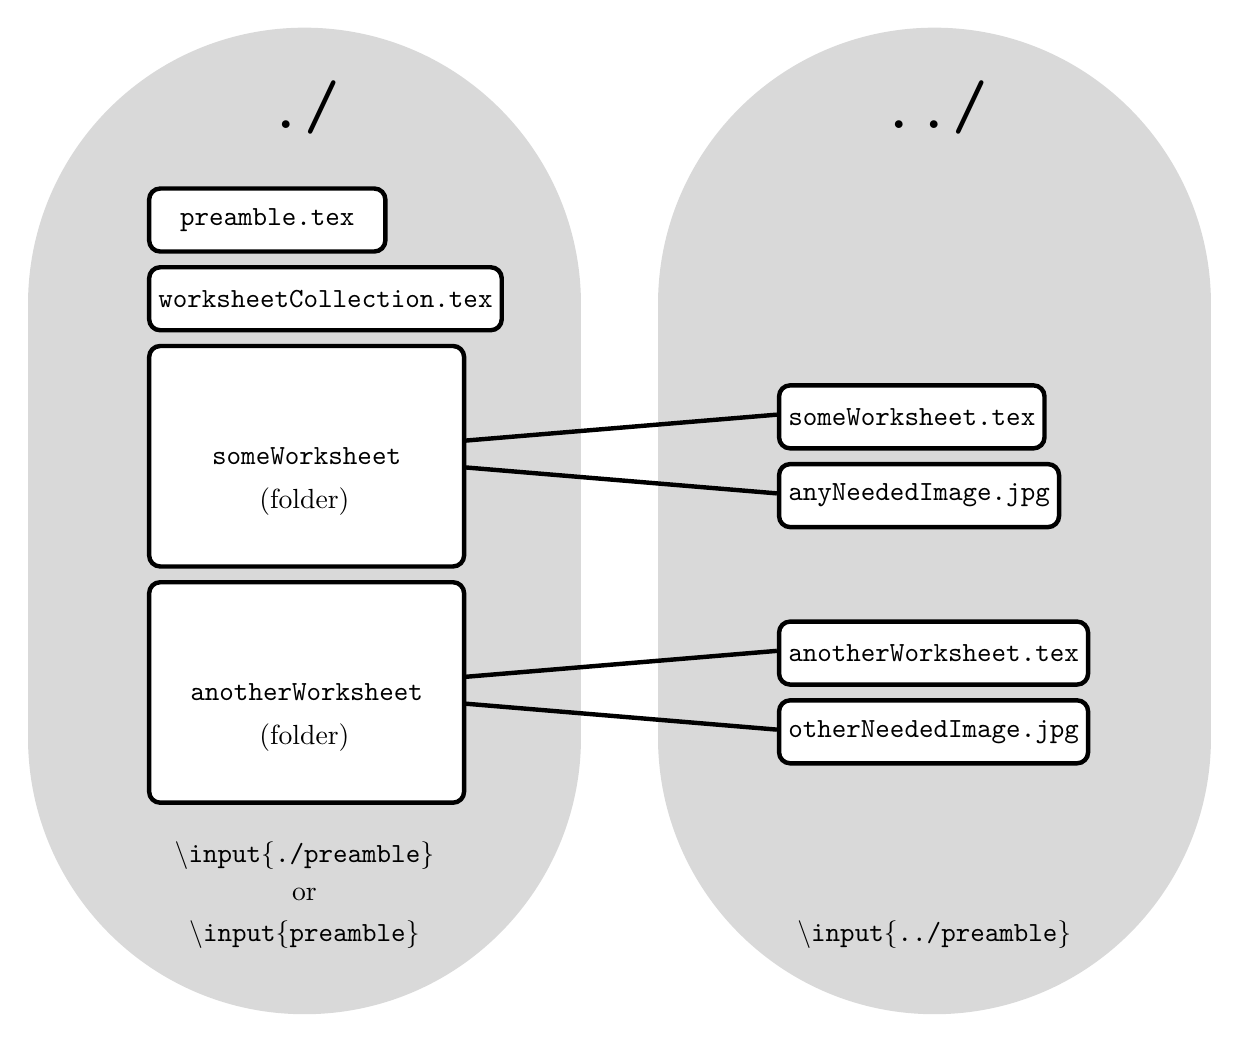
\begin{tikzpicture}
      % Define styles for nodes
      \tikzstyle{document} = [anchor=north west,draw, rounded corners,
      rectangle,
      minimum width=3cm,fill=white, minimum height=.8cm, ultra
      thick,font=\ttfamily]
      \tikzstyle{folder} = [anchor=north west,draw, rectangle, rounded corners,
      minimum width=4cm,fill=white, minimum height=2.8cm, ultra
      thick,font=\ttfamily]

      % Thick grey lines
      \draw[line width=200pt,white!85!black,line cap=round] (2,1.5) -- (2,-4);
      \draw[line width=200pt,white!85!black,line cap=round] (10,1.5) --
      (10,-4);

      % Connections
      \draw[ultra thick] (2,-.4) -- (8,.1);
      \draw[ultra thick] (2,-.4) -- (8,-.9);
      \draw[ultra thick] (2,-3.4) -- (8,-2.9);
      \draw[ultra thick] (2,-3.4) -- (8,-3.9);

      % Symbols at top
      \node at (2,4) {\Huge \tt ./};
      \node at (10,4) {\Huge \tt ../};

      % Define the folders at top level
      \node[document] at (0,3) {preamble.tex};
      \node[document] at (0,2) {worksheetCollection.tex};
      \node[folder] at (0,1) {someWorksheet};
      \node[] at (2,-1) {(folder)};
      \node[folder] at (0,-2) {anotherWorksheet};
      \node[] at (2,-4) {(folder)};

      % Define the documents in the worksheets folder
      \node[document] at (8,.5) {someWorksheet.tex};
      \node[document] at (8,-.5) {anyNeededImage.jpg};
      \node[document] at (8,-2.5) {anotherWorksheet.tex};
      \node[document] at (8,-3.5) {otherNeededImage.jpg};

      % paths at bottom
      \node at (2,-5.5) {\tt\textbackslash input\{./preamble\}};
      \node at (2,-6) {or};
      \node at (2,-6.5) {\tt\textbackslash input\{preamble\}};
      \node at (10,-6.5) {\tt\textbackslash input\{../preamble\}};

    \end{tikzpicture}
  }
\end{center}

In this setting, the file \verb!worksheetCollection.tex! might look something
like
\begin{verbatim}
\document{xourse}
%% Where to find images
\graphicspath{  %% When looking for images,
{./}            %% look first at your level,
{./basics/}     %% then in this folder,
}    
\title{My Groovy Worksheets}
\begin{abstract}
  Some of my worksheets.
\end{abstract}
\maketitle
\begin{document}
\activity{someWorksheet/someWorksheet}
\activity{anotherWorksheet/anotherWorkSheet}
\end{document}
\end{verbatim}

The preamble would include:
\begin{verbatim}
%% where to find images
\graphicspath{
{./}
{./someWorksheet/}
}
\end{verbatim}

\section{Exercise banks}

Exercise banks can be made with \verb!xourse! files. If you are making an
exercise bank, you might want to have essentially one exercise per file.

\paragraph{File structure}

\begin{center}
  \scalebox{.7}{
    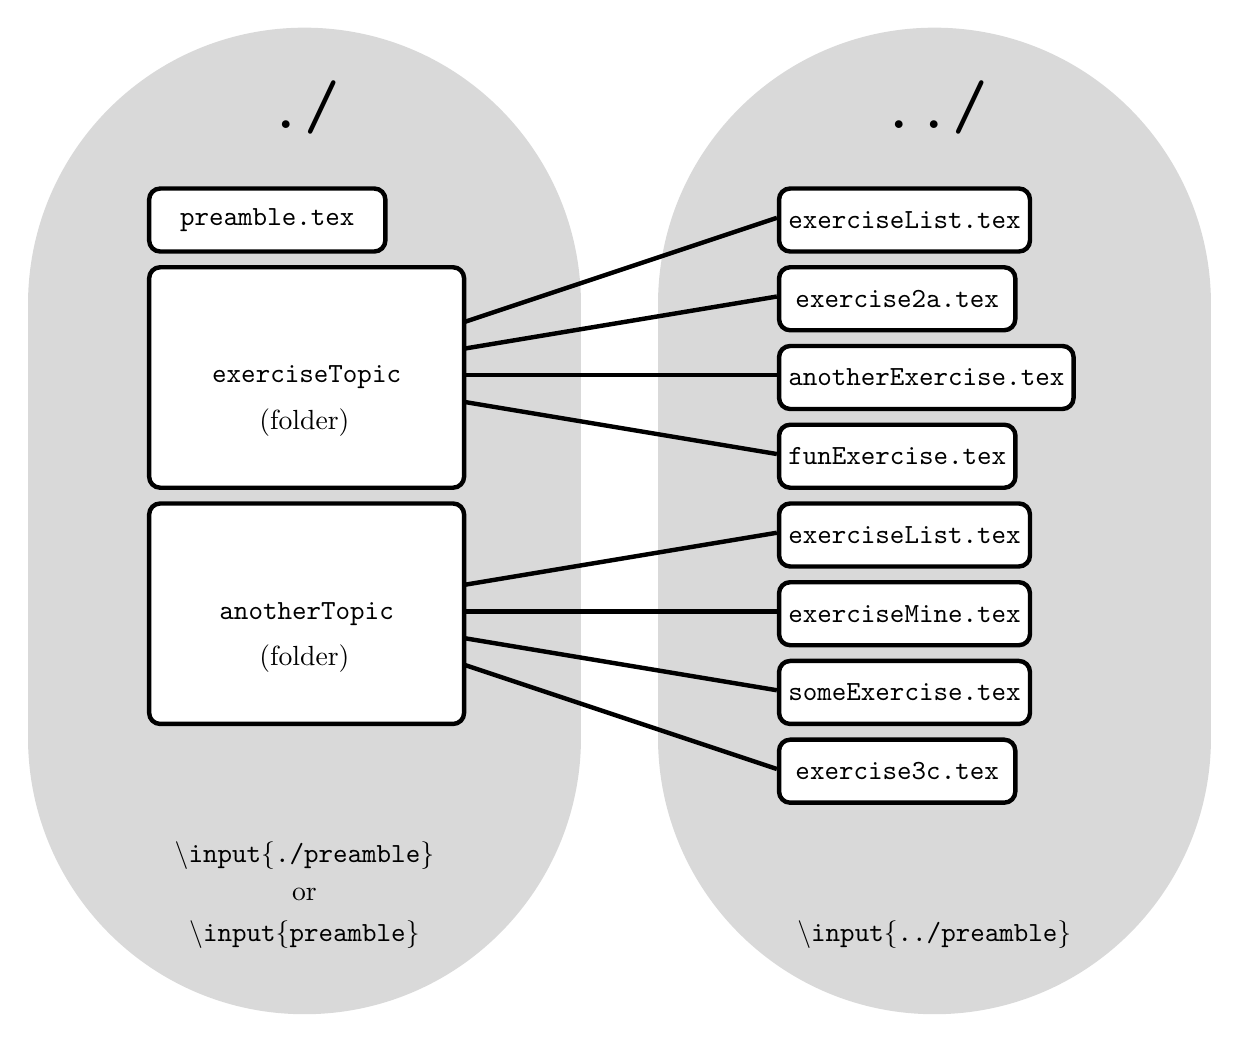
\begin{tikzpicture}
      % Define styles for nodes
      \tikzstyle{document} = [anchor=north west,draw, rounded corners,
      rectangle,
      minimum width=3cm,fill=white, minimum height=.8cm, ultra
      thick,font=\ttfamily]
      \tikzstyle{folder} = [anchor=north west,draw, rectangle, rounded corners,
      minimum width=4cm,fill=white, minimum height=2.8cm, ultra
      thick,font=\ttfamily]

      % Thick grey lines
      \draw[line width=200pt,white!85!black,line cap=round] (2,1.5) -- (2,-4);
      \draw[line width=200pt,white!85!black,line cap=round] (10,1.5) --
      (10,-4);

      % Connections
      \draw[ultra thick] (2,.6) -- (8,2.6);
      \draw[ultra thick] (2,.6) -- (8,1.6);
      \draw[ultra thick] (2,.6) -- (8,.6);
      \draw[ultra thick] (2,.6) -- (8,-.4);

      \draw[ultra thick] (2,-2.4) -- (8,-1.4);
      \draw[ultra thick] (2,-2.4) -- (8,-2.4);
      \draw[ultra thick] (2,-2.4) -- (8,-3.4);
      \draw[ultra thick] (2,-2.4) -- (8,-4.4);

      % Symbols at top
      \node at (2,4) {\Huge \tt ./};
      \node at (10,4) {\Huge \tt ../};

      % Define the folders at top level
      \node[document] at (0,3) {preamble.tex};
      \node[folder] at (0,2) {exerciseTopic};
      \node[] at (2,0) {(folder)};
      \node[folder] at (0,-1) {anotherTopic};
      \node[] at (2,-3) {(folder)};

      % Define the documents in the exercises folder
      \node[document] at (8,3) {exerciseList.tex};
      \node[document] at (8,2) {exercise2a.tex};
      \node[document] at (8,1) {anotherExercise.tex};
      \node[document] at (8,0) {funExercise.tex};

      \node[document] at (8,-1) {exerciseList.tex};
      \node[document] at (8,-2) {exerciseMine.tex};
      \node[document] at (8,-3) {someExercise.tex};
      \node[document] at (8,-4) {exercise3c.tex};

      % paths at bottom
      \node at (2,-5.5) {\tt\textbackslash input\{./preamble\}};
      \node at (2,-6) {or};
      \node at (2,-6.5) {\tt\textbackslash input\{preamble\}};
      \node at (10,-6.5) {\tt\textbackslash input\{../preamble\}};
    \end{tikzpicture}
  }
\end{center}

The individual exercises that live in folders might look something like:

\begin{verbatim}
\documentclass{ximera}
\begin{document}
\begin{exercise}
Compute:
\[
  \frac{\partial}{\partial x} \sin(3xyx) 
  = \answer{3yz\cos(3xyz)}
\]
\end{exercise}
\end{document}
\end{verbatim}

In this case, the \verb!exerciseList! within \verb!exerciseTOpic! might look
like

\begin{verbatim}
\documentclass{xourse}
%% Where to find images
\graphicspath{  %% When looking for images,
{./}            %% look first at your level,
{./basics/}     %% then in this folder,
}    
\title{My exercise banks}
\begin{document}
\begin{abstract}
Here is an exercise bank
\end{abstract}
\maketitle

\practice{exercise2a}
\practice{anotherExercise}
\practice{funExercise}

\end{document}
\end{verbatim}
IF you don't give your \verb!xourse! file a title, it will not show up on the
front page.
Instead you can link directly to the file by going to something like:
\begin{center}
  \verb!https://some.ximera.server/DEPOLOY-NAME/exerciseTopic/exerciseList!
\end{center}

\paragraph{Exercises as part of a course} can be included as a folder within
the section that the exercises address. The next section will address this in
detail.

\pdfOnly{\onecolumn\begin{multicols}{2}}
    \section{Courses}

    This section is about \textit{best practices} when writing an entire
    course.
    \begin{itemize}
      \item Keep related content in the same folder
      \item use \texttt{\textbackslash sectionstyle} and
            \texttt{\textbackslash chapterstyle}
      \item When you give a definition, ask a question after.
      \item When you give and example, give an explanation, with
            \texttt{\textbackslash answer} boxes to fill in.
      \item Think about how you name things
      \item Think about how paths are resolved.
      \item Avoid over sectioning -- make a style and keep it simple.
    \end{itemize}

    \begin{verbatim}
%% where to look for inputs
\makeatletter
\def\input@path{
{./}
{./coverArt/}
{./introduction/}
}
\makeatother
\end{verbatim}
    \pdfOnly{\end{multicols}}

\begin{center}
  \scalebox{.7}{
    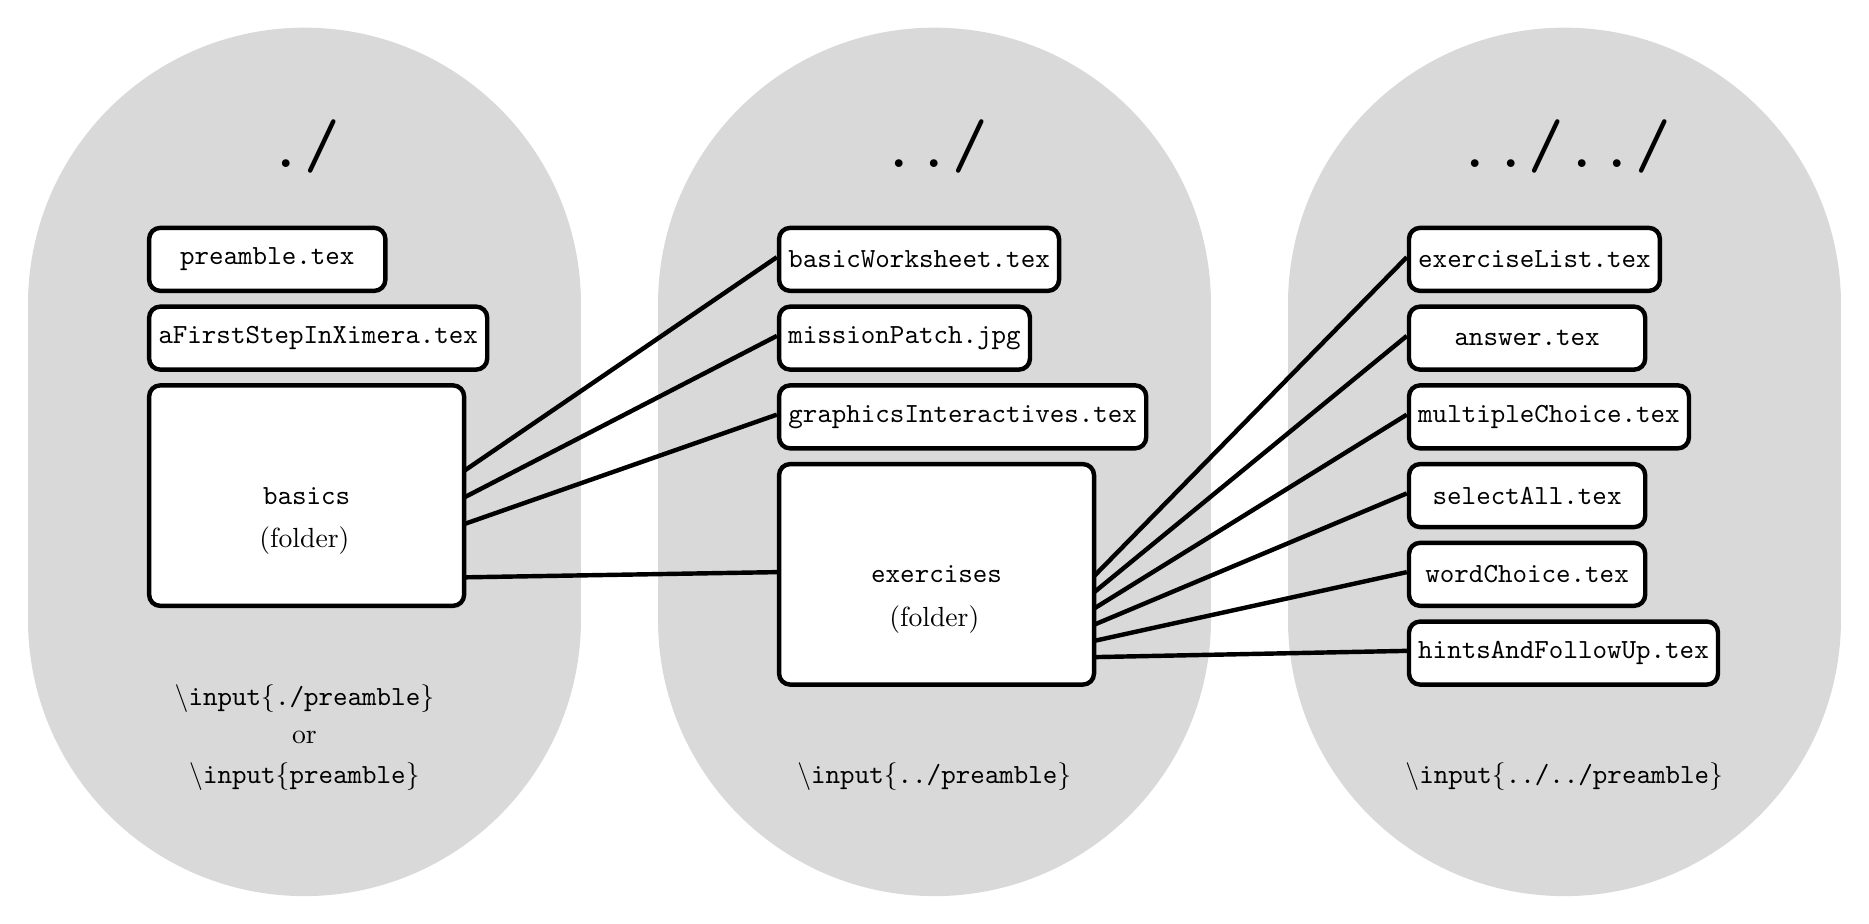
\begin{tikzpicture}
      % Define styles for nodes
      \tikzstyle{document} = [anchor=north west,draw, rounded corners,
      rectangle,
      minimum width=3cm,fill=white, minimum height=.8cm, ultra
      thick,font=\ttfamily]
      \tikzstyle{folder} = [anchor=north west,draw, rectangle, rounded corners,
      minimum width=4cm,fill=white, minimum height=2.8cm, ultra
      thick,font=\ttfamily]

      % Thick grey lines
      \draw[line width=200pt,white!85!black,line cap=round] (2,2) -- (2,-2);
      \draw[line width=200pt,white!85!black,line cap=round] (10,2) -- (10,-2);
      \draw[line width=200pt,white!85!black,line cap=round] (18,2) -- (18,-2);

      % Connections
      \draw[ultra thick] (2,-1.5) -- (8,2.6);
      \draw[ultra thick] (2,-1.5) -- (8,1.6);
      \draw[ultra thick] (2,-1.5) -- (8,.6);
      \draw[ultra thick] (2,-1.5) -- (8,-1.4);

      \draw[ultra thick] (11,-2.5) -- (16,2.6);
      \draw[ultra thick] (11,-2.5) -- (16,1.6);
      \draw[ultra thick] (11,-2.5) -- (16,.6);
      \draw[ultra thick] (11,-2.5) -- (16,-.4);
      \draw[ultra thick] (11,-2.5) -- (16,-1.4);
      \draw[ultra thick] (11,-2.5) -- (16,-2.4);

      % Symbols at top
      \node at (2,4) {\Huge \tt ./};
      \node at (10,4) {\Huge \tt ../};
      \node at (18,4) {\Huge \tt ../../};

      % Define the folders at top level
      \node[document] at (0,3) {preamble.tex};
      \node[document] at (0,2) {aFirstStepInXimera.tex};
      \node[folder] at (0,1) {basics};
      \node[] at (2,-1) {(folder)};

      % Define the documents in the basics folder
      \node[document] at (8,3) {basicWorksheet.tex};
      \node[document] at (8,2) {missionPatch.jpg};
      \node[document] at (8,1) {graphicsInteractives.tex};
      \node[folder] at (8,0) {exercises};
      \node[] at (10,-2) {(folder)};

      % Define the documents in the exercises folder
      \node[document] at (16,3) {exerciseList.tex};
      \node[document] at (16,2) {answer.tex};
      \node[document] at (16,1) {multipleChoice.tex};
      \node[document] at (16,0) {selectAll.tex};
      \node[document] at (16,-1) {wordChoice.tex};
      \node[document] at (16,-2) {hintsAndFollowUp.tex};

      % paths at bottom
      \node at (2,-3) {\tt\textbackslash input\{./preamble\}};
      \node at (2,-3.5) {or};
      \node at (2,-4) {\tt\textbackslash input\{preamble\}};
      \node at (10,-4) {\tt\textbackslash input\{../preamble\}};
      \node at (18,-4) {\tt\textbackslash input\{../../preamble\}};
    \end{tikzpicture}
  }
\end{center}
\pdfOnly{\twocolumn}

\begin{verbatim}
  %% where to find images
  \graphicspath{
  {./}
  {./graphicsVideosAndInteractives/}
  }
  \end{verbatim}

Use a global grpahics path
  \begin{verbatim}
    %% where to find images
    \graphicspath{
    {./}
    {./graphics/}
    {.././graphics/}    
    }
    \end{verbatim}

See page 10 and page 24  



\end{document}